\chapter{\IfLanguageName{dutch}{Stand van zaken}{State of the art}}
\label{ch:stand-van-zaken}

% Tip: Begin elk hoofdstuk met een paragraaf inleiding die beschrijft hoe
% dit hoofdstuk past binnen het geheel van de bachelorproef. Geef in het
% bijzonder aan wat de link is met het vorige en volgende hoofdstuk.

% Pas na deze inleidende paragraaf komt de eerste sectiehoofding.

Dit hoofdstuk bevat je literatuurstudie. In dit onderdeel zal er diep in gegaan worden op het onderwerp. Delen van het onderwerp worden grondig onderzocht om later tot een conclusie te komen. 

\section{Microservices}
\subsection{Definitie}
Een term die vaak zal terug keren in deze paper is 'monolithic'. Deze term betekend het volgende: Bij een monolithic communiceren alle deeltjes van een applicatie met een grote databank of datastore. In een databank of datastore wordt er info en data opgeslaan om dit dan later te gebruiken. De data kan later gebruikt worden om het gepasseerde semester van een bedrijf te analyseren. 
Het artikel van \textcite{Mauersberger2017} geeft meer uitleg over microservices door de moeilijkheden bij een monolithic aan te kaarten. Bij een verandering binnen een monolithic architectuur, wordt er een heel nieuwe versie van de architectuur uitgebracht. Een verandering brengt een hoop extra werk mee. Dit omvat 
\begin{itemize}
	\item De volledige architectuur moet opnieuw getest worden.
	\item Deze architectuur kan heel complex worden bij het toevoegen van functionaliteiten.
	\item De complete architectuur moet opnieuw gedeployed worden bij elke update.
	\item De impact van een verandering kan verkeerd ingeschat worden.
	\item Bij een fout in een proces, kan de volledige architectuur falen.
\end{itemize}
De definitie die te vinden is in dit artikel, gaat als volgt: "A method of developing software applications as a suite of independently deployable, small, modular services in which each service runs a unique process and communicates through a well-defined, lightweight mechanism to serve a business goals.". Als je de definitie leest, zie je drie onderdelen. Het eerste onderdeel vertelt hoe een microservice in elkaar zit. Het is een onafhankelijke, kleine, modulaire services. Modulaire services zijn services waarbij veel delen uitwisselbaar zijn met diverse services. De services staan los van elkaar. Ze hebben geen invloed op elkaar. Daarom zijn ze ook onafhankelijk. Wordt er info gestuurd of gevraagd van services A dan zal dit geen invloed hebben op de andere services. De eenvoudige communicatie is een tweede eigenschap van microservices. Er is nood aan communicatie omdat sommige services wel data moeten uitwisselen om hun 'job' te kunnen doen. De communicatie kan gebeuren op verschillende manier. De manier die gekender is, is 'Messaging via a Message Broker'. Dit wil zeggen dat microservice A een bericht plaats op de wachtrij bij microservice B wanneer die data wil doorsturen. Dan kan microservices B aan die data wanneer hij die nodig heeft. Ze zullen soms moeten wachten maar ze zijn zo goed als onafhankelijk van elkaar. De derde eigenschap omvat dat een microservice wordt gemaakt in functie van een requirement uit de business. Elk product in de business heeft een doel dat moet voldoen aan eisen. Het unieke aan microservices is dat we ze gaan bekijken vanuit de eisen binnen de business. Het doel van microservices is, de problemen die te vinden zijn bij een monolithic, verhelpen. De vorige definite legde uit wat microservices zijn. Dit artikel zegt waar men microservices kan plaatsen. Er is dus één groot framework. Daar zitten meerdere onafhankelijke services in.

\begin{figure}[h]
	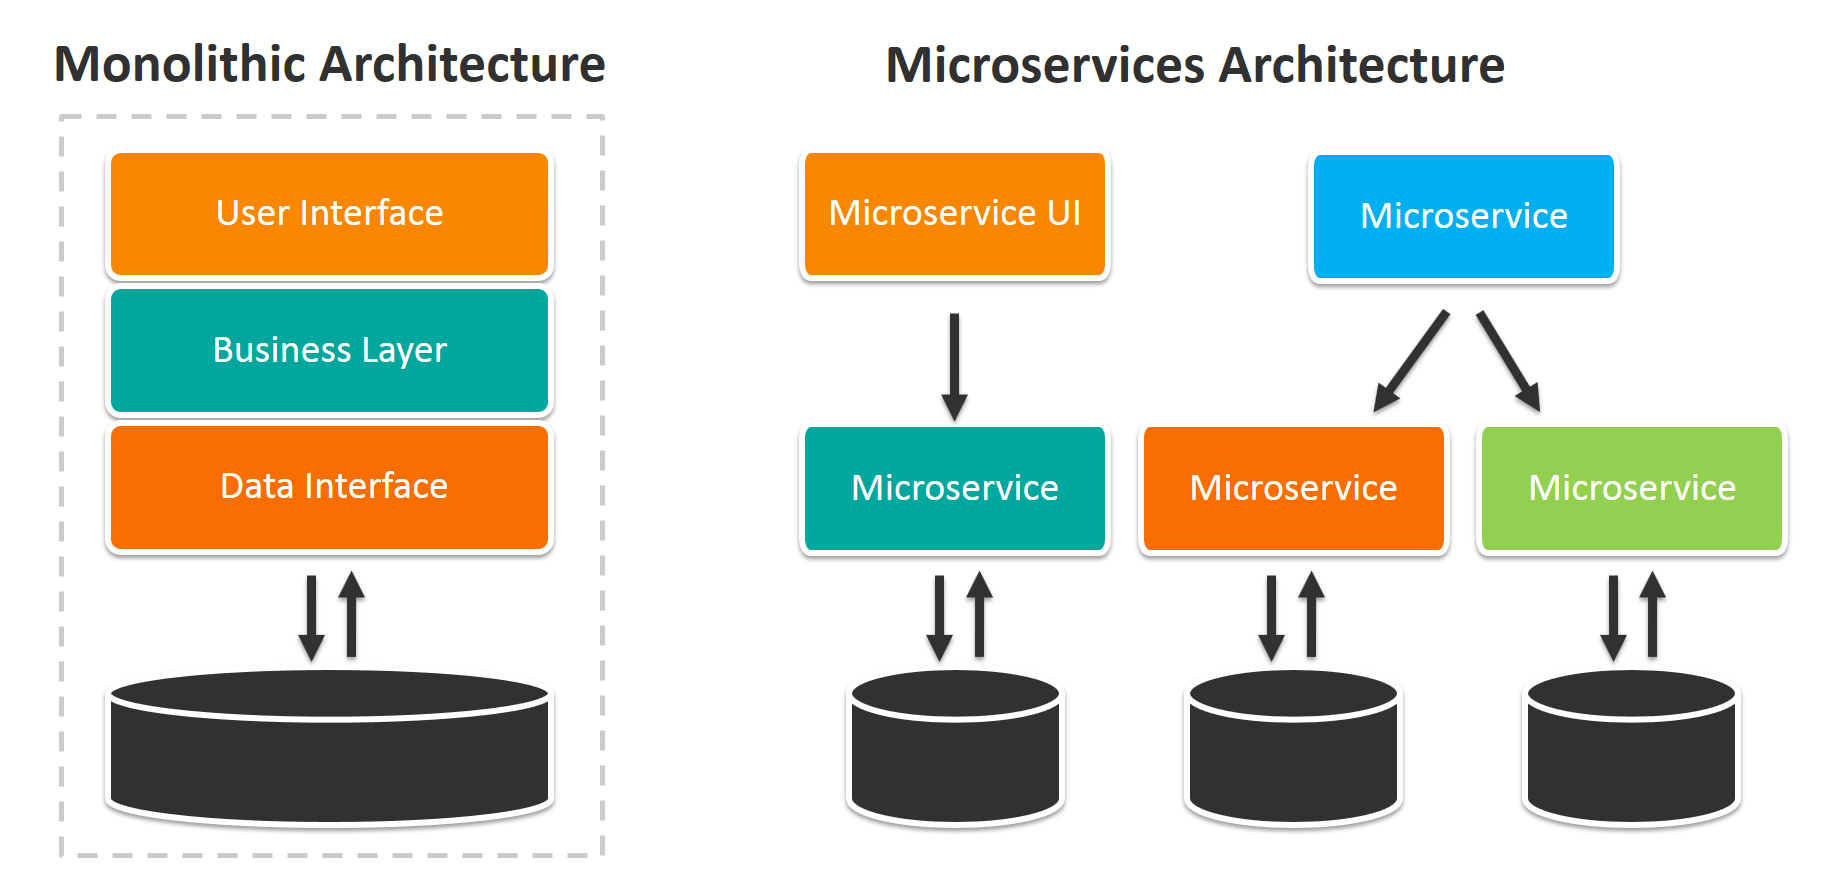
\includegraphics[width=10cm]{microservices-vs-monolithic.jpg}
	\centering
	\caption{Een monolithic architectuur naast een microservice architectuur. \textcite{Watts2018}}
\end{figure}
Figuur 2.1 is afkomstig uit artikel \textcite{Watts2018}.
Zoals te zien in figuur 2.1 is er een groot verschil tussen een monolithic architectuur en die van een microservice. De monolithic wordt weergegeven in de linkerkant van de foto. Aan de rechterkant van de foto is een voorbeeld te zien van een microservice architectuur. Daar is duidelijk te zien dat elke microservice een eigen databank/datastore heeft. Voor elke functionaliteit wordt een microserives aangemaakt, die dan nog eens apart een databank voor zich krijgt. Als bij microservice A een probleem is dan heeft dit niet meteen impact op de andere services. De communicatie tussen microservice A en de anderen zal wel hinder ondervinden. Maar de andere microservices kunnen wel nog steeds onafhankelijk verder. 
Het artikel van \textcite{series2018} bestaat uit elf verschillende onderdelen. Eerst wordt er uitleg gegeven over wat microservices zijn. Dit is hun definitie van microservices: "A software architecting pattern that allows software to be developed into relatively small, distinct components. Each of the components is abstracted by an API(s) and provides a distinct subset of the functionality of the entire application". Ook hier zien we weer het puntje passeren dat een microservice een klein componentje is van een groter geheel. Die eigenschap wordt heel hard benadrukt. Na het uitleggen van microservices, schrijven ze ook over hoe microservices zo scalable zijn. Met scalable bedoelen ze schaalbaarheid. De mogelijkheid van software om mee te groeien als het aantal gebruikers vermeerderd. Dus eigenlijk dat de software nog steeds even goed presteerd bij 10 gebruikers als bij 2 000 gebruikers. Ook lichten ze toe hoe belangrijk API's zijn binnen een microservice architectuur. API's zijn een set van definities die ervoor zorgen dat deeltjes in een programma met elkaar kunnen communcieren. Een voordeel van API's is dat je niet moet weten hoe de andere code werkt. Verder wordt er ook gepraat over de verschillen tussen een monolithic architectuur en een microservice architectuur. 


\textcite{Benetis2016a} vertelt dat microservices uit dezelfde ideologie kotmt als Agile en DevOps. DevOps is een samenvoegsel van development en operations. Bij deze methode ligt de nadruk op de samenwerking en communicatie tussen verschillende partijen. Hier zijn de partijen de software engineers en andere IT specialisten. Deze ideologie omvat het volgende: het afbreken van kleine, traag evoluerende architectuur of monolithic en deze in microservices steken. Zoals te zien is in figuur 2.2. We zien dat de monolithic alle puntjes in een kader heeft. Dit staat symbolisch voor het grote geheel dat eigen is aan een monolithic. Alles zit samen in één grote doos. Maar bij microservices is dit niet zo, daar zit elk deeltje/requirement in een aparte doos. 
\begin{figure}[h]
	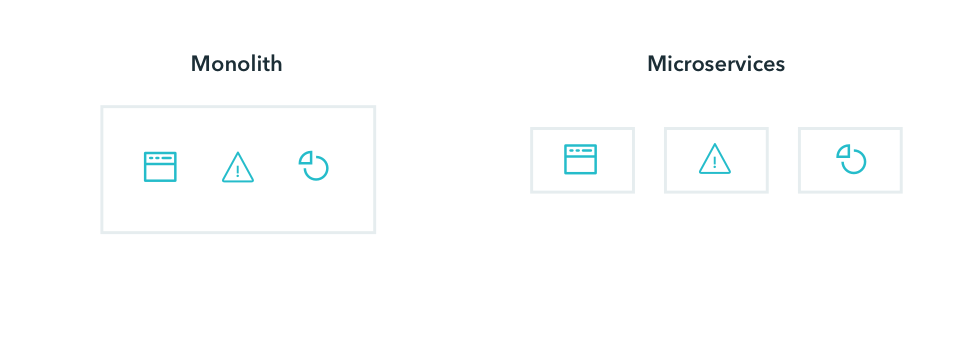
\includegraphics[width=10cm]{Mono_Micro.png}
	\centering
	\caption{Een monolithic vergeleken met een microservice. \textcite{Benetis2016a}}
\end{figure}


\subsection{Het belang van microservices}
Bij een monolithic kan het aanpassen van een deeltje, veel werk vragen. Dit werd meer uitgelegd bij de definite van microservices. Microservices spelen gemakkelijker in op het periodieke opleveren van delen software. Deze technologie legt niet heel het framework plat als er deeltjes moeten bij gecodeerd worden. Microservices kunnen sneller inspelen op de Agile analyse/ontwikkel methode. Dit is ook een reden waarom microservices zo een opkomst kent. De analyse methode Agile werkt met periodieke opleveringen die kunnen gaan van twee weken tot een maand. In de periode wordt er gewerkt aan een functionaliteit of een eis van de klant. 
\textcite{series2018} haalt aan dat microservices van belang zijn bij het scalen van software.
In het artikel van \textcite{RDX2016} worden er verschillende eigenschappen aangekaart. Microservices moeten een doel in de business vervullen. Naast dit, zorgt microservices er ook voor dat bescherming eenvoudig wordt. 
Zoals te vinden is in het artikel van \textcite{Troisi2019} zijn er acht manieren hoe microservices bescherming bieden. 
De verschillende manieren zijn:
\begin{itemize}
	\item Het gebruik van OAuth voor gebruikers identificatie en wat de gebruiker kan.
	\item Gebruik bescherming in de diepte om een prioriteit toe te kennen aan service keys.
	\item Schrijf zelf geen krypto code.
	\item Update je bescherming tijdig.
	\item Maak gebruik van een firewaal met gecentraliseerde controle.
	\item Zorg dat je 'onctainers' niet in een publiek netwerk te vinden is. 
	\item Maak gebruik van software om virussen te vinden.
	\item Monitor alles.
\end{itemize}
Als eerste puntje is er 'het gebruik van OAuth voor gebruikers identificatie en wat de gebruiker kan.'.  OAuth/OAuth2 is een protocol voor authorisatie. Het is een gemak om gebruik te maken van een protocol. Een protocol zijn een aantal regels om te communiceren tussen computers. 
Een andere manier is om in de diepte bescherming te voorzien. Dit kan verwoord worden als bescherming steken in verschillende lagen van een systeem. Er moet worden nagegaan welke deeltjes het kwetsbaarst zijn en daar dan op verschillende lagen van beveiliging op toepassen. 
Microservices maken het toepassen van deze methode, eenvoudiger. Doordat er gefocust kan worden op beveiliging. Het framework maakt het gemakkelijker om de verschillende lagen vast te stellen. Als ze binnen zijn bij een van de microservices zijn ze niet binnen in het volledige systeem. 
Een manier dat wordt afgeraden is om je eigen crypto code te schrijven. Er zijn genoeg open source alternatieven. Enkel bij heel uitzonderlijke redenen wordt een eigen crypot code geschreven. 
Een belangrijk punt is het automatisch regelmatig updaten van de beveiliging. Als er updates komen in de software van beveiliging, moeten die ook uitgevoerd worden. Het automatiseren van die updates, kan veel werk besparen achteraf. Dit wordt dan ook best gedaan bij het begin van microservices. Bescherming binnen software is niet meer een nice to have maar een must have. Ook een firewal is deze dagen een must. Het biedt ook meer controle aan aan de gebruiker. 
Een andere manier van bescherming is om je containers uit het publieke netwerk te halen. Dit is eigenlijk zorgen dat gebruikers je achterliggende architectuuur niet kunnen zien. Ervoor zorgen dat erna maat één toegangspoort is.  Hier kan een vorige manier ook bijgestoken worden. Microservices kunnen achter een firewall gestoken worden als bescherming. 
Als er met containers wordt gewerkt, moet er ook beschemring aanwezig zijn. Een container is een plek waar kleine deeltjes code kunnen op gedeployed worden. 
De laatste manier spreekt voor zich verder in deze thesis. Monitor alles, komt nog aan bod.
Het artikel van \textcite{Watts2018} geeft het belang van een microservice goed weer. Microservices beschermen het gehele systeem, bij een goede implementatie. Het toepassen van de agile methode is eenvoudiger bij microservices dan bij een monolithic. Met deze technologie is het eenvoudiger om een aanpassing te testen en te onderhouden. Niet de volledige architectuur moet opnieuw getest worden bij een aanpassing. Als team A een aanpassing doet aan hun microservice, zullen de andere teams geen hinder ondervinden. 

Een belangrijk aspect van microservices is de authenticatie en de authorisatie. In het artikel van  \textcite{Ayoub2018} worden beide aspecten goed aangehaald. Het is een moeilijkheid om op een uniforme manier veiligheid, bescherming, authorisatie en authenticatie toe te passen op microservices. Authenticatie is bevestigen dat jij het bent. Dit wordt gedaan via een gebruikersnaam en een wachtwoord. Authorisatie is wat je kan doen met een programma. Bijvoorbeeld een beheerder van een site kan meer dan een bezoeker. 
\begin{figure}[h]
	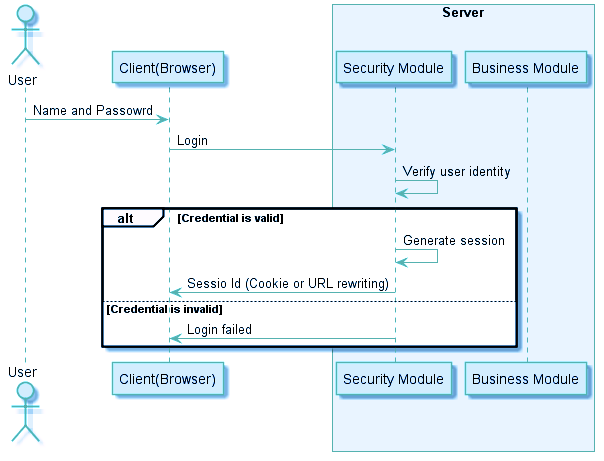
\includegraphics[width=10cm]{monolithic_auth.png}
	\centering
	\caption{Een diagram van authenticatie bij een monolithic. \textcite{Ayoub2018}}
\end{figure}
Zoals te zien is op bovenstaande afbeelding, figuur 2.3, wordt de authenticatie afgehandeld binnen het monlithic proces. Wanneer de gebruiker inlogt, wordt de beveiligings module aangesproken. Deze kijkt of de gebruiker een bekende is, of er al gegevens in de databank zitten. Als het aanmelden gelukt is, wordt er een sessie gecreëerd. Een sessie wordt opgeslaan aan de hand van cookies. Cookies worden op je computer geplaatst door je browser. Het zijn kleine tekstbestanden. De sessie onthoudt wie je bent aan de hand van een ID. Dit zorgt ervoor dat je je niet elke keer opnieuw moet aanmelden als je van pagina verandert.  Elke keer dat de bezoeker van de site iets doet, wordt de sessie ID samen gestuurd met de request. Een request is een aanvraag. Als het ID correct is, weet de site dat de gebruiker ingelogd is. Bij elke aanvraag wordt de ID meegestuurd zodat er kan gecontroleerd worden of die zo wordt de authenticatie bij een monolithic afgehandeld.
Wanneer er gekeken wordt om authenticatie toe te passen bij microservices, komen volgende puntjes veel voor:
\begin{itemize}
	\item In elke microcservice moet er authenticatie en authorisatie afgehandeld worden. Het beste wordt dit toegepast op een uniforme manier. Dan wordt er van uit gegaan dat er in elke microservices een stukje code gaat komen dat herbruikt wordt. Maar dit zorgt ervoor dat elke microservice toch afhankelijk is. Bij het uitkomen van een nieuwe versie, moet dit deeltje dan weer geüpdate worden. Dit heeft invloed op de flexibiliteit van het framework.
	\item "Single responsibility" zijn twee woorden die microservices mooi omschrijven. Een microservice omvat een stukje business logica. De algemene logica van authenticatie en authorisatie mag niet in een microservices gegoten worden. 
\end{itemize}
In het algemeen zijn authenticatie en authorisatie een complex onderdeel van microservices.
Er zijn vijf oplossingen volgens dit artikel.
\begin{itemize}
	\item Distributed session manangement,
	\item client token,
	\item single sing-on, 
	\item client token with API gateway.
\end{itemize}
Distributed Session management is de eerste oplossing. Het managen van een sessie over microservices. Dit kan op verschillende manieren. Aan de hand van Sticky sessions. Dit houdt in dat alle requests van één gebruiker naar dezelfde server worden gestuurd. Dan kan men ervan uitgaan dat de gebruikte data van die specifieke gebruiker is. Of men kan dit toepassen via session replication. Dit houdt in dat alle instanties de sessie data synchronizeren. Deze manier van toepassen heeft als nadeel dat er veel overhead zal zijn op het netwerk. Een andere methode is centralized session storage. Dit omvat dat bij het aanspreken van een microservice, deze de gebruikers data gaat ophalen van op een gedeelde plaats. 
Een andere manier om authenticatie en authorisatie toe te passen is via een client token. Een token wordt gebruikt om aan te tonen dat je ook echt de gebruiker bent. Een token wordt bijna altijd onleesbaar gemaakt. Het klinkt bijna hetzelfde als een sessie. Het verschil ligt hem in het feit dat een sessie op de server centraal wordt bijgehouden. Een token wordt bijgehouden door de user zelf.
Naast de Distributed session management en client token is er ook nog single sign-on. Na een enkele aanmelding, kan de gebruiker alle microservices gebruiken binnen de applicatie. 
Een andere manier is een client token wiht API gateway. Deze manier is gebaseerd op de client token. Maar nu is er een API gateway toegevoegd aan het begin van een externe request. Dit zorgt ervoor dat het framework niet zichtbaar is aan de buitenwereld. 
\subsection{Algemene aanpak om microservices te implementeren}
Het interessante artikel van \textcite{Benetis2016} over een 6-stappen plan om microservices te implementeren. Een paar woorden die meer verklaring nodig hebben voordat we verder gaan. Een gateway is een netwerkpunt dat dient als toegang tot een ander netwerk. Een gateway is een soort toegangspoort. Implementatie is een procesmatige invoering van een verandering of vernieuwing. Iets implementeren of vernieuwen. 

In grote lijnen is dit het zes-stappen plan. Als eerste komt aan bod "serve a business purpose". Hierna komt "protect your stuff". Eens dat gebeurt is, zegt het artikel "see no evil, hear no evil". Dan komt "find your stuff" aan bod. Hierna wordt de volgende stap "create a gateway" aangehaald. Als laatste komt "construct events" aan de beurt. 
Bij eerste stap, "Serve a business purpose", zegt de titel al veel van wat er verwacht wordt. Een microservices is gebaseerd op een business requirement. En niet het doel dat het IT-team voor ogen heeft. Een voorbeeld van een business requirement is het ophalen van data om die dan te analyseren om daar later dan conclusies uit te trekken. Dit kan in een microservices gegoten worden. Eens het doel voor ogen is bij een microservices, moet er ook gekeken worden naar wat de microservices moet kunnen. Zo lang het bij enkele microservices blijft, is automated deployement etc. niet zo belangrijk. Maar eens we gaan scalen en meerdere microservices in één systeem steken zouden volgende puntjes toch self-sufficient moeten zijn:
\begin{itemize}
	\item Geautomatiseerde implementatie
	\item Blootstelling aan andere systemen, toegankelijk eindpunt
	\item Opslag van data
	\item Schaalbaarheid en belasting
\end{itemize}
Zoals te zien is op figuur 2.2, is een microservices één klein deeltje in een groot geheel. Later in dit stappenplan zal de figuur ook uitgebreidt worden en zal het geheel duidelijk worden. 
\begin{figure}[h]
	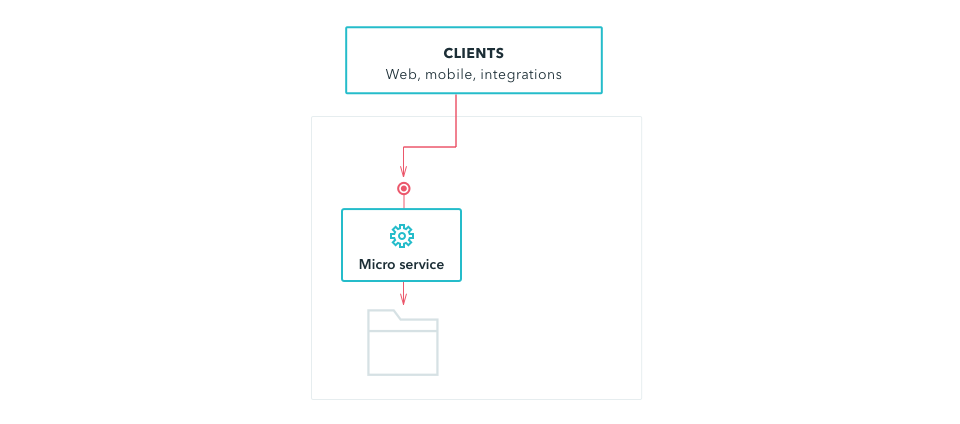
\includegraphics[width=10cm]{1.png}
	\caption{Een microservice dat voldoet aan een business requirement. \textcite{Benetis2016}}
	\centering
\end{figure}

Na "Serve a business purpose" komt "Protect your stuff". Dit gaat over de bescherming van een microservices. Als het gaat over bescherming moet dit op elk moment gebeuren. Ookal heb je maar één à twee microservices, of honderden, bescherming is belangrijk. Het is belangrijk op over al de microservices een uniforme manier te vinden om ze te beschermen. De bescherming kan een requirement op zich zijn, dus ook dit kan in een microservices worden gestoken. Bescherming is een vage term daarom een korte uitleg van hoe een bescherming er zou kunnen uitzien. De meest bekende manier is natuurlijk authorisatie en authenticatie. Authorisatie is het verkrijgen van rechten om bijvoorbeeld een product toe te voegen op een site. Authenticatie is het aanmelden op facebook bijvoorbeeld. De controle of jij het wel echt bent. Een manier op de microservices te beschermen is gecentraliseerde session opslag. Hier zal verder in de thesis nog dieper op worden ingegaan. Kort uitgelegd betekend gecnetraliseerde session opslag dat de data van de user centraal opgeslagen staat. Zodat alle microservices de zelfde session data lezen en gebruiken. 
\begin{figure}[h]
	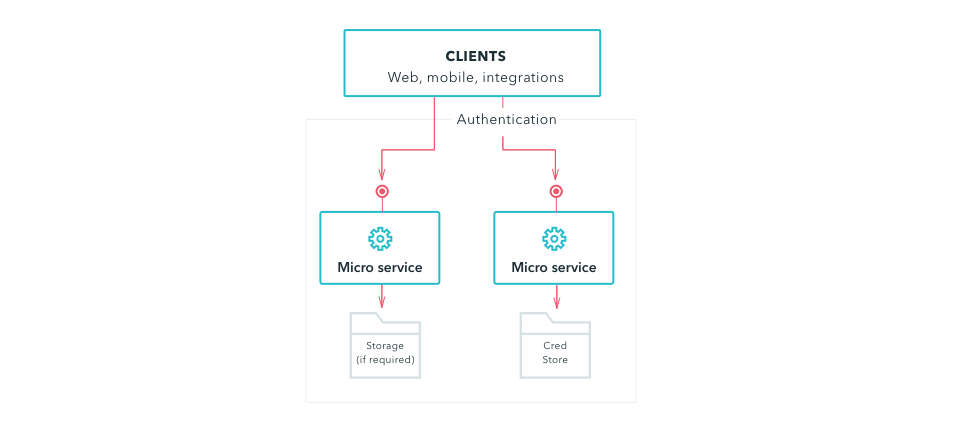
\includegraphics[width=10cm]{2.png}
	\caption{Een microservice waar bescherming aan is toegevoegd. \textcite{Benetis2016}}
	\centering
\end{figure}
In figuur 2.3 is de authenticatie in een microservices gestoken. 

Na de eerste twee stappen komt "See no evil, hear no evil". Eens de microservice is opgezet en gedeployed, moet er gemonitord worden. Daarmee wordt bedoeld dat hoe de microserivces zich gedraagd goed moet bijgehouden worden. Alles zou goed moeten gelogd worden, zodat bij een probleem het geen moeite is om te vinden waar het probleem zich voordeed. Ook hier is het aangeraden om doorheen het hele systeem een uniforme manier van loggen aan te houden. Ook kan men hiervan een microservice maken. Dit wordt ook afgebeeld in figuur 2.4.
\begin{figure}[h]
	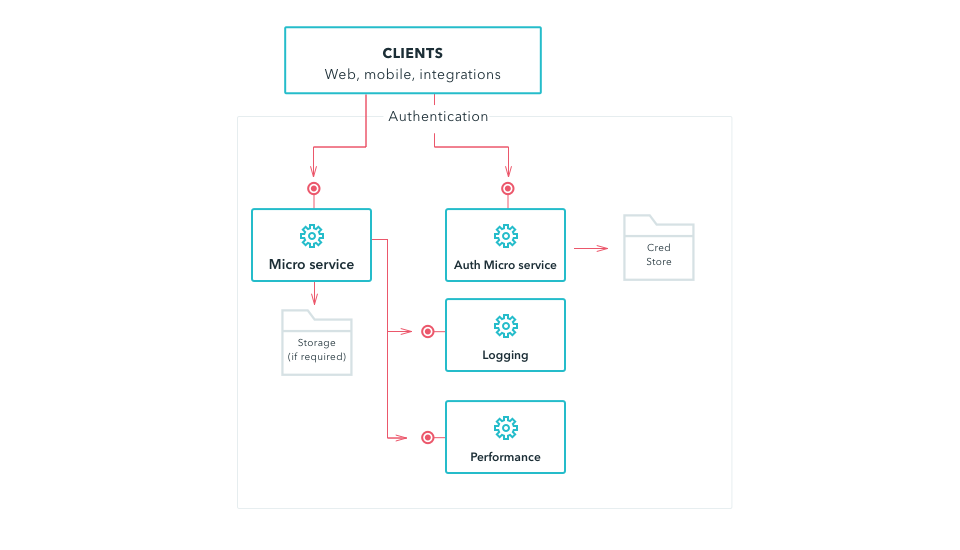
\includegraphics[width=10cm]{3.png}
	\caption{Een microservice waar er monitoring is aan toegevoegd om chaos te voorkomen. \textcite{Benetis2016}}
	\centering
\end{figure}

Als vierde stap komt er "Find your stuff". In deze stap wordt er gezocht naar een manier om de microservices met elkaar te communiceren. Hiermee wordt bedoelt hoe dat microservices A gegevens vraag aan microservices B. Die dat dan ook vraagt van een andere microservice. Een veel gebruikte techniek hiervoor is "service registry". Een service registry is een databank waar alle services met hun instanties en locatie woren opgeslaan. Daar worden dan ook connecties in opgeslaan. Ook hier wordt er aangeraden om dat in een microservices te gieten. Zodat ook hiervan het gedrag kan gemonitord worden. In figuur 2.5 zie je hoe de service registry kan toegevoegd worden. In de figuur is die terug te vinden onder de naam "service discorvery".
\begin{figure}[h]
	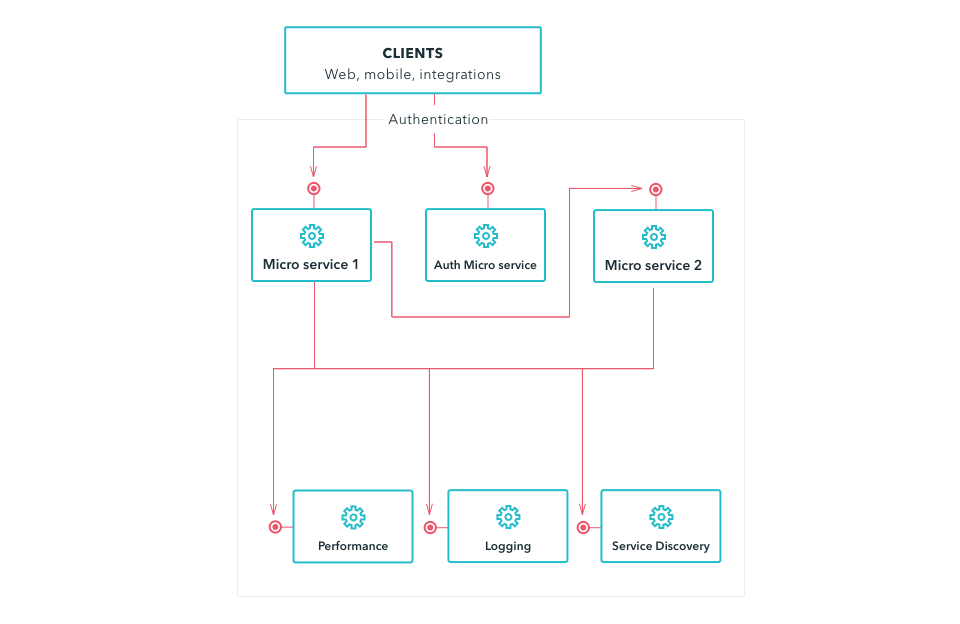
\includegraphics[width=10cm]{4.png}
	\caption{Een microservice dat authenticatie als bescherming toepast. \textcite{Benetis2016}}
	\centering
\end{figure}

Nu is er een service, bestaande uit microservices, dat beschermd is en kan doen wat het zou moeten doen. Maar niet de  volledige service moet open en bloot gelegd worden. En daar zorgt stap 5, "Create a gateway", voor. Een API gateway kan een scherm zijn waar je gegevens op invult en mogelijke acties op doet en die spreken dan de correcte microservices aan. De taak van een gateway is voornamelijk zorgen dat request/aanvragen naar de juiste microservice worden doorgestuurd. Andere taken van een API gateway kunnen volgende zijn
\begin{itemize}
	\item Beveiliging: een API gateway kan de binnenkomende aanvragen valideren. 
	\item Prestatiegegevens kunnen geregistreerd worden.
	\item Omzetten van aanvragen in enkele of meerdere microservices.
	\item Abstractie van de clientinterface. Wanneer er van microservice verandert wordt, moet er niet van interface/scherm verandert worden. 
\end{itemize}

In figuur 2.6 is te zien hoe zo een API gateway kan worden toegepast. Zo is ok te zien dat de authenticatie microservice er niet inzit. Die wordt apart gehouden. De request naar de authenticatie mogen niet langs de API gateway gaan. Omdat ze dan zo meteen 'binnen' zitten. Pas na authenticatie mag men request sturen naar de API gateway.
\begin{figure}[h]
	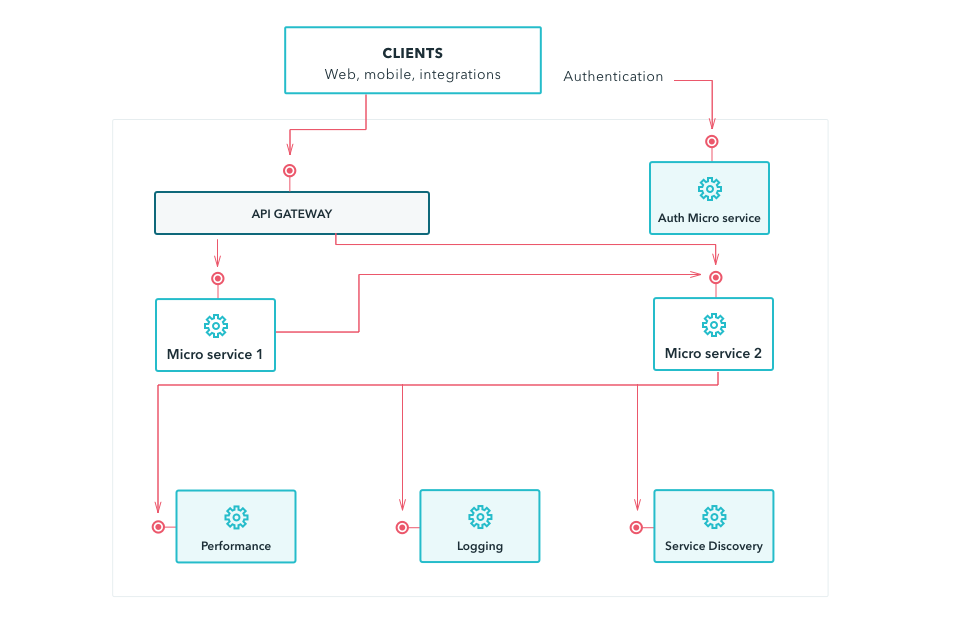
\includegraphics[width=10cm]{5.png}
	\caption{Een microservice dat een gateway gebruikt. \textcite{Benetis2016}}
	\centering
\end{figure}

Nu is er al een deftige architectuur aanwezig. Stap 6, "construct events", zal het plaatje dan ook compleet maken. De meeste microservices vragen aan asynchrone oplossing. Een niet-gelijktijdige verwerking van aanvragen. Een manier om asynchroon te werken, is werken met een queue of wachtrij. Een bekende manier om asynchroniteit toe te passen is publish/subscribe pattroon. Dit wil zeggen dat microservice A zijn berichten of data op een wachtrij gaat zetten. De microservices die data of berichten van microservice A moeten ontvangen, gaan zich abonneren op die wachtrij. Dus vanaf het moment dat microservice A iets op die wachtrij plaatst, krijgen de geabonneerden een melding en kunnen ze het bericht of de data gaan ophalen. Enkele voordelen van dit als asynchrone oplossing te gebruiken:
\begin{itemize}
	\item Taken inplannen. Dit kan door deze gewoon op de wachtrij te plaatsen met een timestamp van wanneer deze moet gebeuren of door een wachtrij te maken voor geplande events.
	\item Abonneren op bepaalde events.
	\item Het asynchrone systeem laten bloot leggen zodat externe klanten verschillende notificaties kunnen handelen.
\end{itemize}
In figuur 2.7 wordt de volledige architectuur weergegeven. Daar wordt er ook mooi afgebeeld hoe men events pland. Als event A voor event B moet gebeuren dan zetten ze die zo op de wachtrij event A voor event B. Want een wachtrij werkt volgens het FIFO (first in first out) principe.
\begin{figure}[h]
	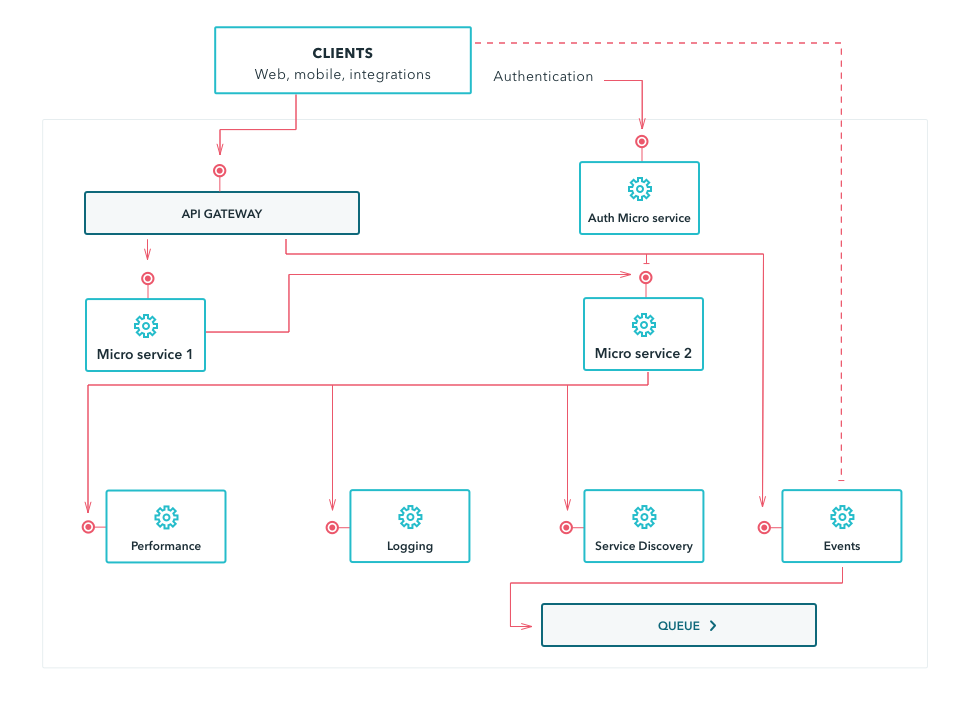
\includegraphics[width=10cm]{6.png}
	\caption{Een microservice met asynchronisatie. \textcite{Benetis2016}}
	\centering
\end{figure}

\textcite{Benetis2016a} beschrijft dat over volgende puntjes goed moet worden nagedacht voordat men de overschakeling maakt naar microservices:
\begin{itemize}
	\item Heeft de organisatie de microservice architectuur wel nodig?
	\item Zijn de juiste competenties aanwezig? Microservices zijn in het algemeen complexer dan een monolithic. Zeker omdat dit iets nieuws is. 
	\item  Staat iedereen achter deze verandering?
\end{itemize}
Eens de beslissing gevallen is om over te schakelen, moet er beslist worden hoeveel de infrastructurele vernadringen van de scope inpalmen. Het verloop om microservices te creëeren gaat als volgt in dit artikel. Eerst het uit elkaar trekken van het bestaande systeem, om het dan in microservices te steken, is een goed begin. Zo moet er constant nagedacht worden over de algemene infrastructuur. Een groot valluik in het begin van het proces is een proof of concept maken. Dit eindigt meestal in een infrastructuur dat niet overeenkomt met de waarden van microservices. Het probleem ligt dan meestal bij een onduidelijke scope. De business requirements zijn meestal wel duidelijk, dit geldt dan meestal niet voor niet-functionele requirements. Daarnaast moeten ook nog volgende stappen gerealiseerd worden:
\begin{itemize}
	\item Bescherming.
	\item Deployment automatisatie.
	\item Loggen en monitoren van microservices hun gedrag.
\end{itemize}
Velen komen niet tot deze stap, door de onderschatting van de overschakeling naar microservices.
\subsection{De voordelen en nadelen van microserivces}
In het artikel van \textcite{series2018} wordt er veel lofzang gedaan over microservices. Het gebruik van microservices zou ervoor zorgen dat de architectuur flexibeler wordt. Met flexibeler wordt bedoelt dat de architectuur zich kan 'aanpassen' of kan inspelen op verschillende situaties. Er kunnen microservices hergebruikt worden. Dankzij microservices is het hermodeleren, implementeren van nieuwe technologieën, ... 
Kleinere deeltjes zijn gemakkelijker te documenteren. De snelheid van microservices zijn een groot pluspunt. Hiermee wordt er geprobeert om aan te halen dat microservices sneller reageren omdat zo kleine, onafhankelijke services zijn. Ze moeten geen 'onnodige' stappen maken om de wens van de klant te vervullen. 
\textcite{Watts2018} geeft enkele voordelen van een microservice. Een developer is onafhankelijk. Ze hebben vrijheid. Ook het scalen van een microservice is veel eenvoudiger. Dit komt door dat microservices minder resources nodig hebben dan een volledige monolithic. Resources zijn hulpbronnen. Zoals al vaak aangehaald in deze bachelorproef, zijn microservices onafhankelijk en zouden ze daarom ook geen hulpbronnen nodig mogen hebben. Binnen een monolithic zijn deeltjes afhankelijk van elkaar en hebben elkaar dus nodig om goed te kunnen functioneren. De deeltjes binnen de monolithic hebben elkaar dus nodig en mogelijk als hulpbron. Een ander voordeel is bij het falen van een microservices, de andere microservices er geen last van zullen hebben. Dit komt door hun onafhankelijkheid. 
\textcite{Benetis2016} geeft aan dat volgende puntjes voordelen zijn van microservices:
\begin{itemize}
	\item Sneller en gemakkelijker developen.
	\item Het refactoren van deeltjes is eenvoudiger door de onafhankelijkheid van de services. 
	\item De schaalbaarheid is eenvoudiger dan bij een monolithic. We kunnen microservices gewoon 'klonen' of kopieëren. 
	\item Het deployen van een onderdeel gaat sneller omdat het team gespecialiseerd is in die bepaalde service.
	\item Als er iets faalt dan is de impact veel kleiner dan bij een monolithic. Dit komt ook door de onafhankelijkheid van de services. 
\end{itemize}
Maar om ervoor te zorgen dat dit allemaal vlot verloopt moeten er ook aanpassingen binnen in het bedrijf/ de organisatie gebeuren. 
\begin{itemize}
	\item Een project zal ingedeeld moeten worden in kleine requirements. De scope zal gedetailleerder moeten zijn.
	\item De teams zullen kleiner moeten worden gemaakt. Zodat er meer op de Agile methode kan gewerkt worden. 
	\item Er zal een sterke band komen met DevOps. Dit komt omdat veel services volledige automatische deployment vragen.
	\item Ook de communicatie tussen de services zal beter moeten worden uitgedacht.
	\item Documenteren is belangrijk. Dit is niet enkel het geval voor microservices maar ook voor elk project.
\end{itemize}
\subsection{Voorbeelden}
In dit deeltje zal je meer te weten komen over hoe grote technologische bedrijven microservices toepassen en hoe ze naar deze technologie zijn overgeschakeld.
Een term die hier vaak zal gebruikt worden, is een monolithic. Dit is de tegenhanger van microservices. Sommige zweren bij monolithic en anderen hebben gouden woorden voor microservices. De beslissing om één van de twee technieken te kiezen, ligt bij wat je precies nodig hebt. Wat de business nodig heeft. 

\subsubsection{Amazon}
\textcite{Mauersberger2017} gaf een voorbeeld waarom Amazon overstapte. Zoals veel grote bedrijven is Amazon begonnen met een grote monolithic. Een van de nadelen die Amazon ondervond aan deze technologie is de moeilijkheid van het inschatten van de zwaarte op de servers. Daardoor verloor Amazon veel geld en was er nood aan herstructurering.
\textcite{Fulton2015} legt ook uit waarom Amazon is overgeschakeld. Het blijkt dat Amazon in 2001 de grootste monolithic was in de retail business. Doordat Amazon een snel groeiende onderneming was, werd de monolithic architectuur heel ingewikkeld. Amazon hun aanpak was, gooi wat je hebt niet weg maar maak het eenvoudiger. 
\subsubsection{Apple}
\subsubsection{Facebook}
\subsubsection{Netflix}

\section{Order-to-cash proces in SAP}
\subsection{Definite}
\textcite{Wong2018} legt uit wat een order-to-cash proces inhoudt. Dit proces heeft veel invloed op het succes van een bedrijf. Ook het het veel invloed op de relatie met de klant. Een voordeel met de huidige technologie is dat het mogelijk is om het proces volledig te automatiseren. Dit heeft veel zorgt voor een minimaal aan fouten en vertragingen. Ook de data en gegevens die worden opgehaald en geanalyseerd is correcter. 
Het proces begint bij het plaatsen van een order door de klant. Alles wat ervoor zorgt dat de klant een order plaatst behoort tot branding, marketing of sales. De hoofdactiviteit van deze afdelingen ligt bij customer relationship, iets wat plaatsvindt voor het OTC proces. Het maakt er geen deel van uit. 
Velen denken dat een OTC is afgerond wanneer de inning heeft plaatsgevonden. Maar er zijn nog belangrijke stappen die gebeuren na het innen van het geld. Onder andere de data die verzameld is tijdens het proces moet geanalyseerd worden om zo het proces te optimaliseren. 
\begin{figure}[h]
	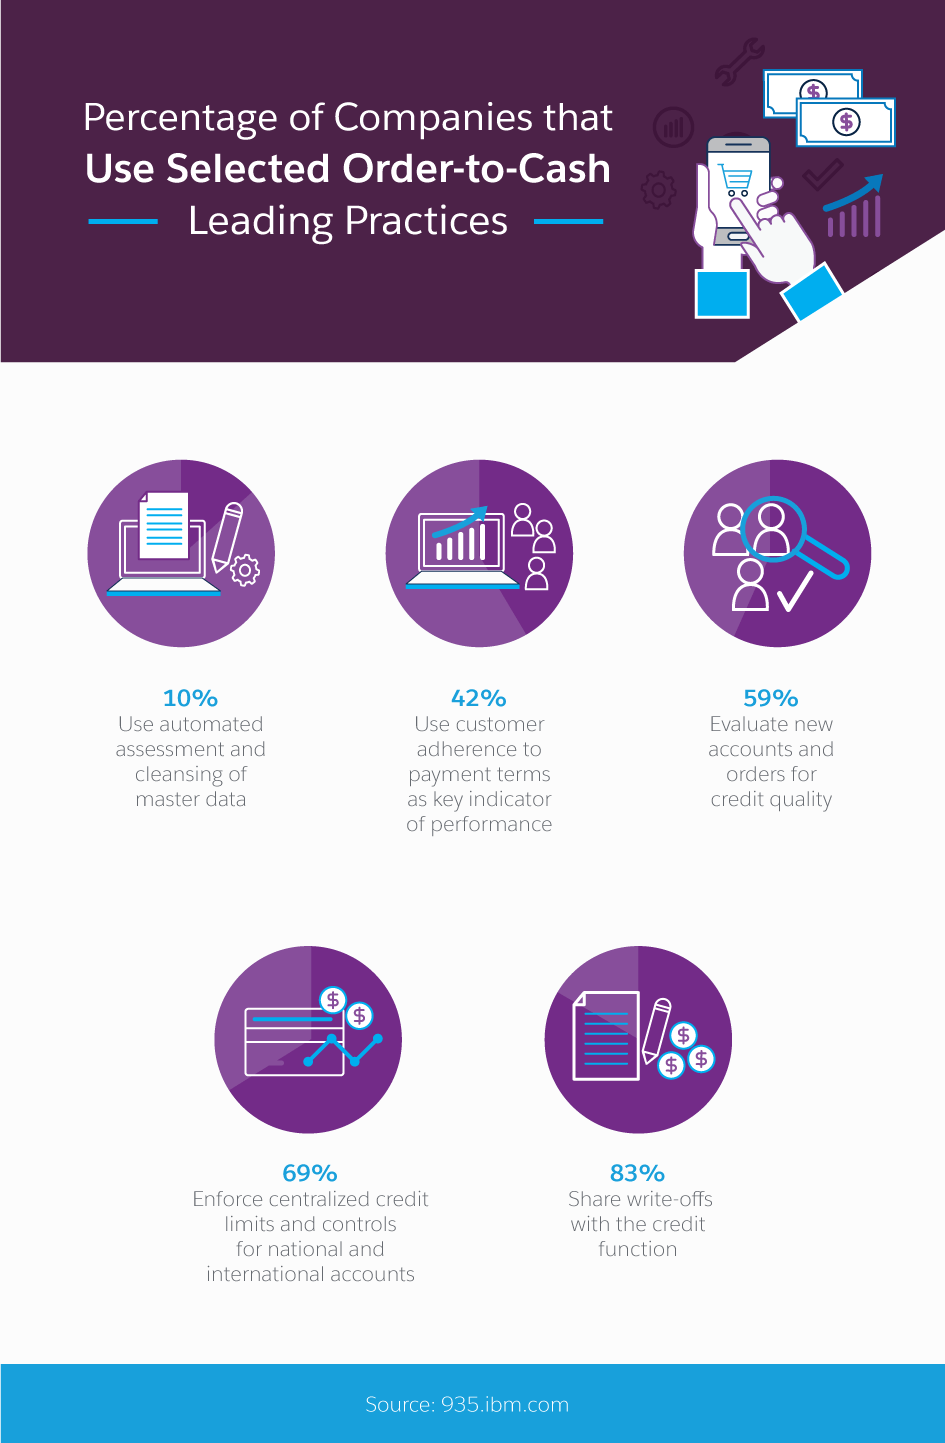
\includegraphics[width=10cm]{wong.png}
	\caption{Het percentage van van bedrijven dat gebruik maken van order-to-cash proces. \textcite{Wong2018}}
	\centering
\end{figure}
Het OTC proces heeft invloed op volgende delen van het bedrijf:
\begin{itemize}
	\item Supply chaing management
	\item Voorraadbeheer
	\item Human resources
	\item Financiële afdeling
\end{itemize}
Zijn er problemen in één van die afdelingen, kan dit voor vertraging zorgen in de andere afdelingen. Bij vertragingen van betalingen of inningen kan zorgen voor een minder goede cash flow binnen het bedrijf. 
Een goed OTC proces maakt indruk op de buitenwereld. Doordat het OTC goed gemanaged wordt, wordt er een beeld gecreërd dat het bedrijf stabiel is. 
Ook bij een OTC is technologie cruciaal. Elk deeltje van het proces kan beter worden door de nieuwe technologie. Er zijn verschillende onderdelen nodig om het proces te optimaliseren om accurate en real-time informatie te verkrijgen. Zoals: 
\begin{itemize}
	\item Gegevens die onderling verbonden zijn.
	\item Automatisering
	\item digitale facturatie
	\item Digitale verzending van het management.
\end{itemize}

Volgende acht stappen komen voor in een OTC proces:
\begin{itemize}
	\item Order management
	\item Credit management
	\item Order fulfillment
	\item Order shipping
	\item Facturatie
	\item Accounts receivable
	\item Inning van het geld
	\item Rapportering en data management
\end{itemize}
In figuur X wordt het afgebeeld in een schema.
\begin{figure}[h]
	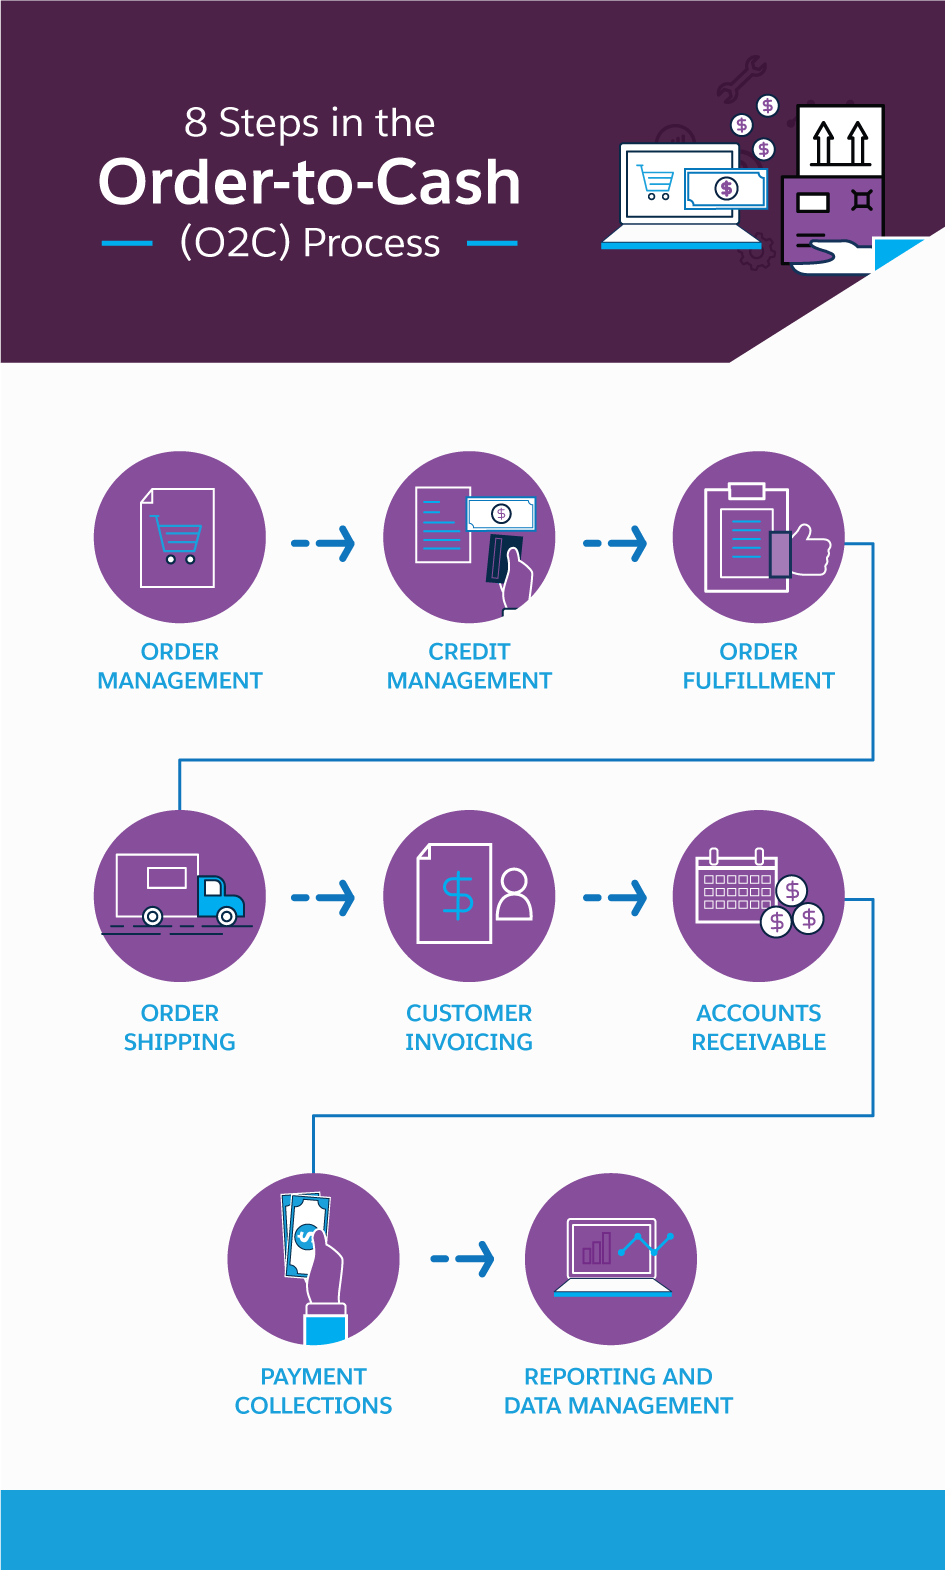
\includegraphics[width=10cm]{wong2.png}
	\caption{Het order-to-cash proces. \textcite{Wong2018}}
	\centering
\end{figure}
Order management is de eerste stap in het proces. Dit begint wanneer de klant een order plaatst. De manier waarop is niet zo belangrijk. Dit deeltje van het proces moet geautomatiseerd zijn. Bij het plaatsen van een order, moet er een ander onderdeel van het order proces getriggerd worden. Dit moet ervoor zorgen dat het order niet uit het oog verloren wordt. Door de automatisatie worden de andere deelnemende partijen direct ingelicht over het nieuwe order en dit heeft een voordeel als het op tijdig leveren aankomt.
Hierna komt credit management. Dit moet ervoor zorgen dat er minder problemen zijn op het einde van het proces. Credit management houdt in dat men kijkt naar hoe het betalingsgedrag van de klant is geweest. Zijn er nog openstaande facturen, betaald de klant altijd maar na enkele aanmaningen? Door dit gedeelte te automatiseren, kan er bespaard worden op menskracht en geld. Als er toch dieper moet gekeken worden naar het betaalgedrag van een klant, kan dit doorgestuurd worden naar een werknemer die er dan naar kijkt. Maar dat zouden dan enkele klanten hun betaalgedrag moeten nagekeken worden, i.d.p.v. alle klanten die een order plaatsen. 
De klanten die een goed betaalgedrag vertonen, worden doorgestuurd naar de volgende stap: Order fulfillment. In deze stap wordt het order ook echt samengesteld en uit de 'rekken' gehaald. Het is een groot voordeel als ook dit gedeelte geautomatiseerd is. Bij het verkopen van een product moet de voorraad automatisch aangepast worden. Eens de producten van het order samengebracht zijn gaan we over naar de volgende stap, order shipping. De verzending van de goederen. De verzending moet goed opgevolgd worden om mogelijke vertragingen te minimaliseren. De gegevens die vrijkomen bij een verzending, moeten zo snel mogelijk in het systeem worden ignegeven. Zodat ook dit deeltje van het proces geoptimaliseerd kan worden. 
Na het verzenden van de goederen komt de facturatie. Op dit deeltje heeft credit management veel invloed. Doordat de wanbetalers er in stap twee al zijn uitgehaald, zouden er hier minder problemen voorkomen. Als er hier fouten worden gemaakt, kan dit een sneeuwbal effect veroorzaken. Dit betekend dat één fout een andere fout kan triggeren en zo voorts. Het systeem moet de juiste info verkrijgen van de werknemers. De info bevat meestal volgende puntjes:
\begin{itemize}
	\item Order specificaties
	\item De kosten
	\item Credit terms
	\item Order datum
	\item Verzendingsdatum
\end{itemize}
Die puntjes moeten ingevoerd worden zodat het facturatiesysteem geautomatiseerd kan worden. Zodat ook hier vertragingen en fouten kunnen geminimaliseerd worden. Eens de factuur is uitgestuurd, wordt er een betaling verwacht binnen een bepaalde periode. Het systeem zou dit ook moeten bijhouden en ervoor zorgen dat er een melding gestuurd wordt nog voor de betalingsperiode is afgelopen. Dit valt onder de volgende stap accoutns receivable. Deze stap probeert om te voorkomen dat mensen vergeten te betalen. 
De volgende stap is payment collections. Wordt een factuur niet betaald binnen de gevraagde periode dan wordt er een aanmaning gestuurd en wordt dit ook in het systeem bijgehouden. De werknemers moeten ook de klanten contacteren zodat ze een reden kunnen geven voor het mogelijks vergeten van de betaling. 
Als laatste stap komt reporting en data management aan bod. Er bestaan programma's om ervoor te zorgen dat performance data over elk deeltje van het proces wordt opgehaald. Door achteraf deze data te gaan analyseren, kan er veel duidelijkheid komen van waar het verkeerd loopt. 

\textcite{PEARSON2017} beschrijft waarom het zo belangrijk is om een goed OTC proces te hebben. Vroeger waren de eisen van de klanten minder hoog. Als klanten iets bestellen, willen ze het de volgende dag al in huis hebben. Er zijn ook voor- en nadelen aan een OTC proces. Als het proces goed opgezet is, kan dit zorgen voor blijere klanten, minder wanbetalers, ... 

Maar is het order management proces niet goed opgezet dan kan het heel snel slecht gaan. Klanten zullen niet tevreden zijn. 
Veel voorkomende redenen van ontevreden klanten:
\begin{itemize}
	\item Orders zitten er dubbel in.
	\item Er zit vertraging tussen de verschillende onderdelen van het proces.
	\item De levering klopt niet met wat er gefactureerd wordt.
	\item Een slecht voorraadbeheer waardoor niet aan de beloften zoals leveringstijd kan voldaan worden.
\end{itemize}
Om zulke problemen op te lossen moet men eerst gaan zoeken van waar die problemen komen. Automatisering is hier een goede oplossing voor. Dordaat verschillende processen aan elkaar gelinkt zijn, is er minder ruimte voor vertragingen. Enkele best practices omvatten:
\begin{itemize}
	\item Minimaliseren van werknemers die handmatig gegevens moeten invullen.
	\item Klanten de mogelijkheid geven om hun bestellingen online te maken.
	\item Integratie van de informatie over het gehele proces.
	\item Elimineren van onnodige moeilijkheden binnen in het proces.
\end{itemize}

Ook het tweede subproces, bill-to-cash proces, heeft pitfalls en best practices.
In volgende opsomming komen verschillende signalen aan bod waaraan te zien is dat het bill-to-cash proces niet goed in elkaar zit.
\begin{itemize}
	\item Het aantal verkoopsovereenkomsten met speciale eisen van de klant is groot. bivjoorbeeld meer dan de helft heeft een uniek verkoopsovereenkomst.
	\item Herhalend aanbiedingen en toegevingen moeten doen door fouten in het proces.
	\item Wat op dee oorspronkelijke offerte stond, werd niet gefactureerd, er werd meer aangerekend.
	\item Een groot aantal creditnota's uitgegeven.
	\item Tussen de verkoop, verzending en het facturerings proces zitten informatie gaten.
\end{itemize}
Om dit alles weg te werken moet er goed gekeken worden naar waar de problemen nu zitten. Enkele best practices:
\begin{itemize}
	\item Integreer klantenprofielen in de betalingssoftware.
	\item Integreer de facturatie en betalingsgegevens met elkaar zodat op de factuur de juiste betalingsmethode staat.
\end{itemize}


\subsection{Technologie}
\subsubsection{Onderdelen van een order-to-cash proces}
Er zijn vier grote onderdelen, namelijk:
\begin{itemize}
	\item Voor-verkoopsactiviteiten.
	\item Het order proces.
	\item Order afwerking.
	\item Betaling.
\end{itemize}
Bij de voor-verkoopsactiviteiten verstaan we het contact dat moet worden gemaakt worden met klant. De klant moet overtuigd worden van het product. Na contact komt er al dan niet een offerte. Soms kan er ook van contact rechtstreeks naar een order gaan. 
Het orderproces bevat maar één onderdeel namelijk: de sales order. 
Binnen de order afwerking valt het leveren van goederen, het verzenden van goederen.
\textcite{Kumaran2015} geeft een mooi overzicht van de stappen die een order to cash proces kan bevatten. Zo begint het artikel met een toelichting dat dit proces een core proces is van de business. Dit wil zeggen dat een bedrijf, zonder dit proces, geen winst kan maken. Het is een essentieel onderdeel van zo wat elk bedrijf. Hoe deze vorm krijgt binnen een bedrijf, is heel verschillend. Een OTC proces start met het ontvangen van orders. Daarna kan, dit gebeurt niet overal, er gekeken worden naar het krediet van de klanten. Mag deze klant wel nog een bestelling plaatsen? Hierna wordt het order opgenomen in het systeem. Het product wordt verzonden en geleverd. En als laatste wordt de factuur betaald. Dit is welliswaar het 'perfecte' verloop van een order to cash proces. 
\begin{figure}[h]
	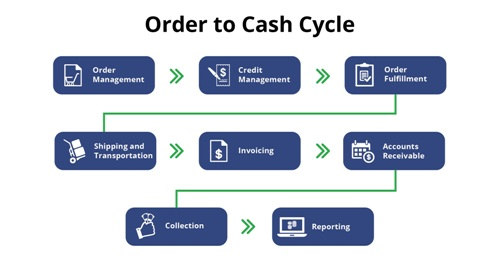
\includegraphics[width=10cm]{Order-to-cash-cycle.jpg}
	\caption{Order-to-cash proces volgens \textcite{Kumaran2015}.}
	\centering
\end{figure}
Er zijn ook enkele uitdagingen verbonden met dit proces. In de volgende opsomming vindt je er enkele:
\begin{itemize}
	\item Hou de orders goed bij, anders loopt het fout vanaf het begin. 
	\item Zonder automatisering verlies je veel tijd. Kostbare tijd.
	\item Zorgen dat de logistiek 'on point' is, is heel belangrijk. Dit is een belangrijk onderdeel binnen het proces.
	\item Bij wanbetalingen, moet de customer service ingrijpen. Ook zij zijn een belangrijk onderdeel van het proces.
\end{itemize}
Het managen van een OTC proces is even belangrijk als de andere aspecten. Een slecht gemanaged proces kan op lange termijn duurder uitkomen dan een onderdeel dat nog niet geautomatiseerd is. 

\textcite{PEARSON2017} vindt dat een OTC proces bestaat uit twee subprocessen. Het order managmenet proces en het bill-to-cash proces. Het laatst vernoemde proces gaat over de facturatie en de inning van het geld.

\textcite{2019} geeft meer uitleg bij enkele termen die in SAP voorkomen. Bij het proces is er een sales team aanwezig. Die spreken met de klant en maken afspraken. Zij zorgen ook voor een deal met de klant. Zij hebben toegang tot informatie over de klant, producten, kwaliteit, prijzen, etc. 
Om ervoor te zorgen dat een order kan verzonden worden, moeten de goederen  opgehaald worden. Die goederen worden opgeslaan in een magazijn. Daar wordt aan order picking en packing gedaan. Bij picking gaat men gaan kijken naar de voorraad om de order te kunnen opvullen. Packing gaat over het inpakken van de goederen tegen beschadigingen. Dit kan door allemaal dozen op een pallet te zetten. Eens de goederen door de fase picking en packing zijn geweest, komt het laden voor transport. De goederen worden dan in containers geladen om dan te verzenden via vrachtwagen of per boot. Hierna komt de facturatie. Dan moet er gewacht worden op de betaling van de klant. Bij laattijdige betaling worden er aanmaningen gestuurd. 
\begin{table}[]
	\resizebox{\textwidth}{!}{%
		\begin{tabular}{|l|p{10cm}|}
				\hline Delivery document & Dit is het leveringsdocument dat gekoppeld is aan een order. Dit wordt uitgestuurd om te bewijzen dat het order geleverd is. \\ \hline
			Picking & Het nagaan of de goederen in de voorraad zitten en ze ook gaan ophalen uit het magazijn. \\ \hline
			Packing & Het inpakken van goederen in dozen, containers, palletten. \\ \hline
			Loading & De goederen inladen in de vrachtwagen of de container. \\ \hline
			Shipment document & Dit document wordt mee afgeleverd met de goederen. Het kan als een soort checklist dienen om na te gaan of alles wel in het afgeleverd pakket zit. \\ \hline
			Shipment cost document & Hierop is de kost terug te vinden van het transport. \\ \hline
			Customer billing document & Dit is een verkoopsdocument, dus dit moet de klant niet betalen. Dit document refereerd naar het delivery document. \\ \hline
			Customer invoice & Dit is de factuur die de klant opgestuurd krijgt. \\ \hline
		\end{tabular}%
	}
	\caption{Tabel met uitleg over termen. \textcite{2019}}
\end{table}


\subsubsection{Wat biedt SAP zelf aan voor microservices}
\textcite{Kyma2019} verteld hoe Kyma in elkaar zit. Dit is een recent project van SAP om toenadering te geven toto microserivces. Kyma is een open-source project gemaakt om Kubernetes. Kubernetes wordt gebruikt om applicaties op verschillende machines te managen. Je kan hiermee cloud-based applicaties en on-premise applicaties omzetten naar een microservice architectuur of naar serverless computing. Cloud-based applicaties zijn applicaties die hun data gaan ophalen over het internet in de plaats van op de harde schijf van de computer. On-premise applicaties zijn de tegenhangers van cloud-based. On-premise is lokaal op de computer, op de harde schijf. Serverless computing gebeurt in de cloud. Dit zorgt ervoor dat er op een dynamische manier de resources van een machine kan aangepast worden. 
Kyma zorgt voor betere end-to-end ervarings scenario's. Die volgen een best-practices voor performance, schaalbaarheid, efficentie en beveiliging. 

\textcite{Semerdzhiev2018} geeft een introductie in het project Kyma van SAP. Binnen SAP wordt er omgegaan met software van verschillende leveranciers. SAP probeert om hun software te customizen naar de wensen van de klant. Dit vraagt meer openheid en een modernere architectuur. 
Het idee achter Kyma is het creëeren van serverless applicaties, mashups en microservices. Ook kan het gebruikt worden om snel kleine, gecustomizede modules te developen. Die modules zijn dan verworven met business logica. 
Er werd iets zoals Knative gemaakt. Knative is een platform dat developers ondersteund om serverless applicaties te maken op Kubernetes. Dit zorgde voor groot enthousiasme bij SAP omdat hun Kyma project een soort van bevesteging keer. Al snel werd Kyma gerefactored om samen te kunnen werken met Knative. Er werden overlappende componenten weggelaten, wat Kyma slanker en gestroomlijnder maakt. Dankzij Knative kan Kyma zich richten op higer-level enterprise applications en service consumption scenario's. En gebruik maken van Knative voor de infrastructuur en development scenario's. 

\textcite{Hofmann2018} geeft het update over de integratie tussen Kyma en Knative. Een toch redelijk belangrijke samenwerking. Beide bieden een complete set van bouwblokken aan. Beiden zijn ook een sterk framework. Bij het gebruik van beide kunnen er could-native oplossingen gebouwd worden op Kubernetes met een sterk framework. Op figuur X is te wat Kyma en wat Knative aanbiedt. 
\begin{figure}[h]
	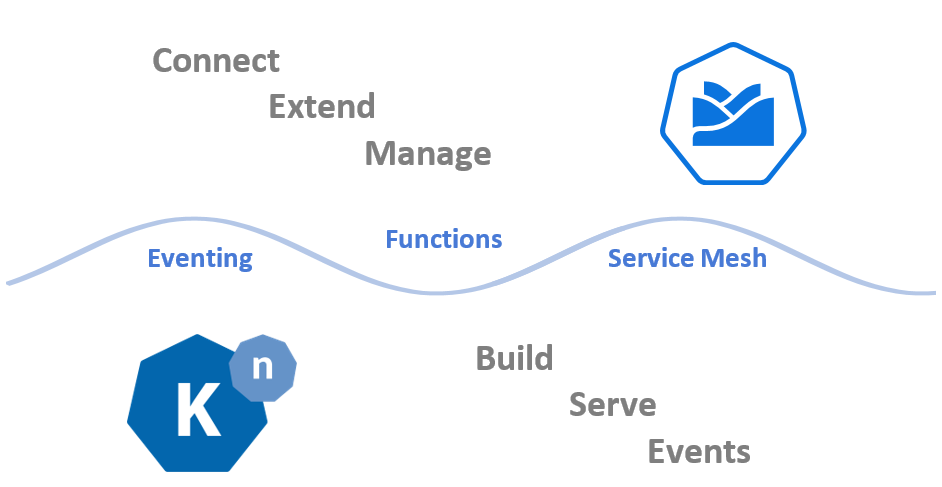
\includegraphics[width=10cm]{1-kyma-knative.png}
	\caption{Wat Kyma, boven de lijn, aanbiedt en wat Knative, onder de lijn, aanbiedt \textcite{Hofmann2018}.}
	\centering
\end{figure}
De laatste maanden werden de repositories gereconstrueerd en daarom zijn er geen tot weinig referenties naar Knative. Naast die grote verandering werd er gewerkt aan een proof-of-concept cloud-native oplossing door het gebruik van Knative en Kyma te samen. 

\textcite{Kannappan2018} schreef een artikel over hoe innovatief izjn met Kyma. Het artikel begint met een eye-opener over Tesla. Hoe innovatief zij wel niet izjn met hun mogelijkheid om de auto's te updaten over-the-air. Tesla heeft bewezen dat innovatie, zelfs in oude branches, nodig is. 
Bij het doormaken van innovatie, zijn er verschillende moeilijkheden die opkomen bij het proces naar digitalisering:
\begin{itemize}
	\item Hetrogene product portfolio: Het aanbieden van één product is verleden tijd. Zeker software bedrijven moeten accepteren dat er diversiteit is en meer nodig is dan één product.
	\item Monolithic deployment: Monolithic applicaties zijn goed maar eens schaalbaarheid erbij komt, worden ze vaak complex. Dit zorgt voor minder vlotte innovatie. 
	\item Cloud-native: Veel bedrijven schakelen over naar "de cloud". Het is geen gemakkelijke stap om alles naar de cloud over te zetten. Het vraagt voor meerdere onderdelen betere oplossingen. Zoals voor de inter-service communicatie, transacties tussen oplossingen, logging over het volledige system.
	\item The need for speed: Het is algemeen geweten dat de snelheid van bijvoorbeeld leveringen een grote rol spelen deze dagen. Ook geldt dit voor software bedrijven. De snelheid waarmee oplossingen kunnen gemaakt worden is belangrijk.
\end{itemize}
Kyma heeft hard gewerkt om deze problemen/uitdagingen te proberen wegwerken. Kyma heeft ook geprobeerd om bedrijven te helpen met de transformatie naar digitalisatie. Kyma geeft bedrijven de mogelijkheid tot:
\begin{itemize}
	\item Be open and extendable: Kyma maakt gebruik van Open Service Broker API specificaties. Dit is een "plug and play" die de mogelijkheid geeft om code te hergebruiken. Ook code van andere partijen te gebruiken. 
	\item Be seamlessly connected: Een eenvoudige manier om een beveiligde connectie te hebben tussen systemen. Deze kunnen gemanaged worden binnen de huidige applicatie om oplossingen te maken in hetrogene landschappen. Eén connectie geeft veel mogelijkheden.
	\item Use any programming language: Developers kunnen in hun geweste programmeertaal coderen.
	\item Bring speed and agility: Er moet niet maanden gewacht worden om use cases of functionaliteiten op te leveren. 
	\item Accelerate innovation: Meestal start dit als een test of een trail. Bij zulke scenario's zijn de kost en de snelheid van zeer groot belang. Dankzij Kyma kunnen bedrijven meteen beginnen werken aan een oplossingen en moet er geen tijd besteed worden aan het zoeken van de best mogelijke oplossing. 
\end{itemize}


\section{Requirements van de business}

